\subsection{Взаимодействие клиента и сервера}
%Взаимодействие клиента и пользователя начинается в тот момент, когда игрок нажимает на кнопку <<Создать игру>>(или <<Подключиться к игре>>). Рассмотрим сценарий варианта использования "Подключение":
  Разработка внутреннего интерфейса программы подразумевает определение команд и функций, необходимых для взаимодействия разных частей проекта. Наилучшим образом это можно отобразить на диаграмме вариантов использования с одним эктором, который объединяет в себе и сервер, и клиента. То есть мы разворачиваем прецеденты <<Отправить сообщение>> и <<Получить сообщение>> из [\ref{fig0}].  

\begin{figure}[ht]
\centering
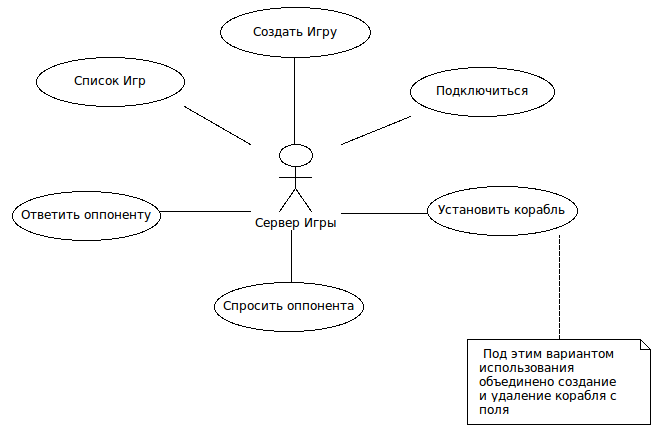
\includegraphics[width=15cm]{images/interface.png}
\caption{Диаграмма прецедентов внутреннего интерфейса}
\label{fig3}
\end{figure}

В данной диаграмме [\ref{fig3}] в качестве эктора представлен сервер игры. Так как интерфейс общения будет одинаков для обеих частей, то интерфейс клиента имеет точно такие же варианты использования. При анализе требований к системе было принято решение реализовывать соединение при помощи сокетов. При этом выделить в отдельный класс процесс, который будет отслеживать новые соединения([\ref{fig14}]). Для каждого нового клиента будет выделяться отдельный поток. Это показано на диаграмме [\ref{fig4}].

\begin{figure}[ht]
\centering
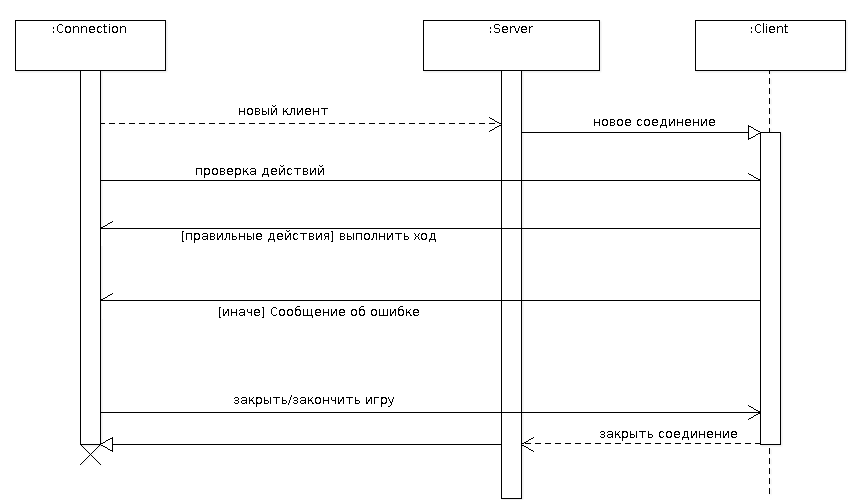
\includegraphics[width=16cm]{images/par.png}
\caption{Диаграмма последовательности сообщений клиент-сервер}
\label{fig4}
\end{figure}

В данной части не представлена диаграмма классов, так как она одновременно описана в 2-х пакетах. К интерфейсу относятся классы Connect и Client, описание которых представлено на рисунках [\ref{fig8}] и [\ref{fig15}] соответсвенно. Дальше мы аналогично будем обращаться к диаграммам из клиентской и серверной частей, так как интерфейс тесно с ними связан.

\begin{figure}[ht]
\centering
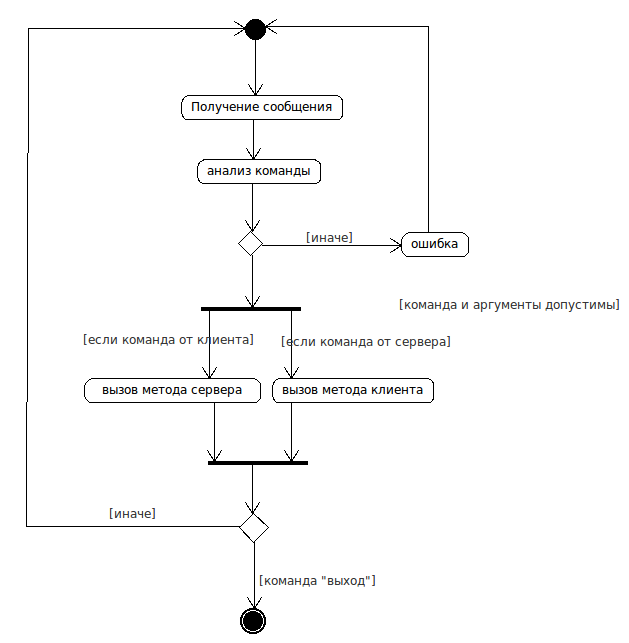
\includegraphics[width=12cm]{images/activity.png}
\caption{Диаграмма принятия сообщения}
\label{fig5}
\end{figure}

На диаграмме [\ref{fig5}] отражена последовательность действий класса, реализующего интерфейс, при получении сообщения от пакета клиента или сервера. В активность <<Вызов метода>> включаются все варианты поведения: передвижение корабля, подключение, создание игры и т.~д., указанные на диаграмме  [\ref{fig3}]. Следует отметить, что процесс получения сообщений непрерывен до тех пор, пока не пришла команда <<Выход>>.

Помимо варианта использования <<Принять сообщение>> [\ref{fig3}], рассмотрен похожий прецедент отправки сообщения. Общий случай которого представлен  на диаграмме~[\ref{fig6}]. В ней нет явных или неявных циклов: при получении  запроса на отправку команды, она тут же уходит; именно по этой причине протокол обмена сообщениями получается асинхронным. 
\begin{figure}[ht]
\centering
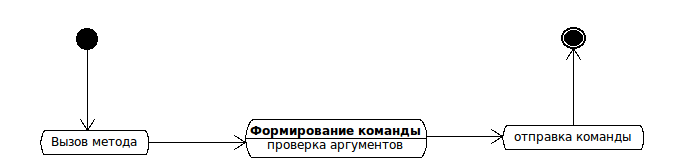
\includegraphics[width=18cm]{images/state1.png}
\caption{Диаграмма отправки сообщения}
\label{fig6}
\end{figure}

В отдельную диаграмму выделен прецедент <<Список Игр>>, который будет обрабатываться отдельным соединением, и его работа представлена на рисунке [\ref{fig7}]. 

\begin{figure}[ht]
\centering
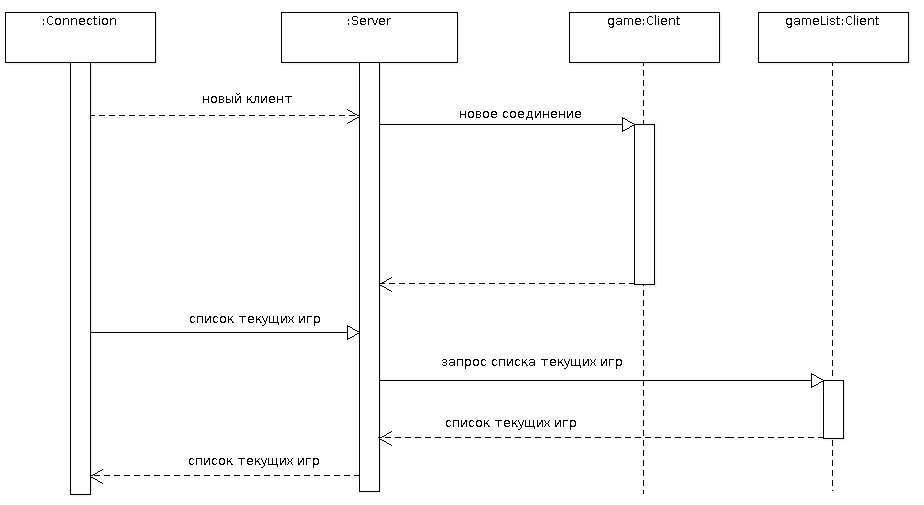
\includegraphics[width=16cm]{images/par2.png}
\caption{Диаграмма запроса списка игр}
\label{fig7}
\end{figure}

На схеме [\ref{fig7}] видно, что для этой операции создается отдельный объект класса Client, жизненный цикл которого завершается, как только он отправляет список текущих игр сервера. Такой ход сделан для того, чтобы сохранить асинхронность протокола.

%Ниже приведены прототипы команд с аргументами, которые должны использоваться клиентом и сервером для общения между собой.
%	\begin{itemize}
%		\item ;
%		\item ;
%		\item ;
%		\item ;
%  	\end{itemize} 
\endinput
